\documentclass[12pt,a4paper]{article}
\usepackage[a4paper, margin=2cm]{geometry}
\usepackage{iftex}
\ifPDFTeX
  \usepackage[T5]{fontenc}
  \usepackage[utf8]{inputenc}
  \usepackage[vietnamese]{babel}
\else
  \usepackage{fontspec}
  \setmainfont{Times New Roman}
  \usepackage[vietnamese]{babel}
\fi
\usepackage{amsmath,amssymb,amsthm}
\usepackage{graphicx}
\usepackage[export]{adjustbox}
\usepackage{algorithm}
\usepackage{algpseudocode}
\usepackage{booktabs}
\usepackage{tabularx}
\usepackage{float}
\usepackage{xcolor}
\usepackage[hidelinks]{hyperref}

\floatname{algorithm}{Thuật toán}
\renewcommand{\algorithmicrequire}{\textbf{Input:}}
\renewcommand{\algorithmicensure}{\textbf{Output:}}
\newcommand{\todo}[1]{\textcolor{red}{\textbf{[#1]}}}

\begin{document}

\begin{center}
    \textbf{TRƯỜNG ĐẠI HỌC CNTT - ĐHQG TP.HCM} \\
    \textbf{KHOA KHOA HỌC MÁY TÍNH} \\
    \vspace{1.5cm}
    \textbf{Môn học} \\
    \textbf{Phân tích và thiết kế thuật toán} \\
    \textbf{(Design and Analysis of Algorithms)} \\
    \vspace{1.5cm}
    {\Large \textbf{BÀI TẬP LỚN}} \\[4pt]
    {\large \textbf{Trực quan hóa thuật toán Quay lui giải bài toán Dò Mìn (WeCode)}}
\end{center}

\vfill
\noindent
\textbf{Assignment:} Bài tập lớn \\
\textbf{Họ và Tên:} Đỗ Quốc Thắng \\
\textbf{MSSV:} 26410111 \\
\textbf{Ngày nộp bài:} 04/10/2026

\newpage
\tableofcontents
\newpage

%=====================================================================
\section{Sản phẩm nộp}

\begin{enumerate}
    \item \textbf{Source code:} thư mục \texttt{app\_minesweeper\_visualizer/}
    \begin{itemize}
        \item \texttt{index.html} --- ứng dụng web trực quan hóa (mở trực tiếp bằng trình duyệt, không cần cài đặt).
        \item \texttt{bai\_tap/WeCode/giai\_do\_min\_wecode.py} --- lời giải nộp trên WeCode.
        \item \texttt{demo/record\_demo.py}, \texttt{demo/capture\_screenshots.py} --- script quay video và chụp hình minh họa.
    \end{itemize}
    \item \textbf{Video demo:} \texttt{demo/demo\_video.mp4} (2 phút 10 giây). Link: \todo{link Google Drive / YouTube}
    \item \textbf{Báo cáo:} tài liệu này.
\end{enumerate}

%=====================================================================
\section{Phát biểu bài toán}

Cho một bảng ô vuông $N$ hàng, $M$ cột. Mỗi ô có thể chứa tối đa một quả mìn. Tại mỗi ô, người ta ghi số lượng mìn nằm ở \textbf{4 ô kề cạnh} (trên, dưới, trái, phải --- hình chữ thập). Biết bảng số, hãy khôi phục vị trí các quả mìn.

\subsection*{Input}
\begin{itemize}
    \item $N, M$: hai số nguyên dương, lần lượt là số hàng và số cột của bảng. \\
    Giới hạn: \todo{bổ sung giới hạn N, M theo đề WeCode}.
    \item $A = (a_{ij})_{N \times M}$: ma trận số nguyên, $a_{ij}$ là số mìn ở các ô kề cạnh với ô $(i, j)$. \\
    Giới hạn: $a_{ij} \in \{0, 1, 2, 3, 4\}$, $\forall i \in [0, N-1], \forall j \in [0, M-1]$.
\end{itemize}

\subsection*{Output}
\begin{itemize}
    \item $B = (b_{ij})_{N \times M}$: ma trận nhị phân, $b_{ij} = 1$ nếu ô $(i, j)$ có mìn, $b_{ij} = 0$ nếu không có mìn, thỏa:
    $$\sum_{\substack{(r, c) \,:\, |r - i| + |c - j| = 1 \\ 0 \le r < N,\; 0 \le c < M}} b_{rc} = a_{ij}, \quad \forall i \in [0, N-1], \forall j \in [0, M-1] \qquad (\ast)$$
    \item Nếu không tồn tại $B$ thỏa $(\ast)$: không xuất gì.
\end{itemize}

\noindent\textbf{Quy ước:} $b_{rc} = 0$ khi $(r, c)$ nằm ngoài bảng.

%=====================================================================
\section{Thiết kế thuật toán}

\subsection{Vét cạn}
Mỗi ô nhận 1 trong 2 giá trị, có $N \cdot M$ ô. \\
Suy ra: không gian tìm kiếm có $2^{NM}$ phương án, mỗi phương án kiểm tra $(\ast)$ mất $\Theta(NM)$. \\
Độ phức tạp: $O(2^{NM} \cdot NM)$. Với $N = M = 10$: $2^{100} \approx 1{,}27 \cdot 10^{30}$ phương án --- không khả thi.

\subsection{Nhận xét: hàng $0$ quyết định toàn bộ bảng}
Xét ràng buộc $(\ast)$ tại ô $(r-1, c)$ với $1 \le r \le N-1$:
$$b_{r-2,\,c} + b_{r,\,c} + b_{r-1,\,c-1} + b_{r-1,\,c+1} = a_{r-1,\,c}$$
Suy ra:
$$\boxed{\,b_{r,\,c} = a_{r-1,\,c} - b_{r-2,\,c} - b_{r-1,\,c-1} - b_{r-1,\,c+1}\,} \qquad (1)$$
Vế phải chỉ chứa các ô thuộc hàng $r-1$ và $r-2$. \\
Suy ra: khi đã biết hàng $0$, áp dụng $(1)$ lần lượt cho $r = 1, 2, \dots, N-1$ sẽ xác định \textbf{duy nhất} toàn bộ bảng.

\noindent Vậy chỉ cần quay lui trên $M$ ô của hàng $0$: còn $2^M$ phương án.

\noindent\textbf{Kiểm tra cuối:} $(1)$ bảo đảm ràng buộc tại các hàng $0, \dots, N-2$. Ràng buộc tại hàng $N-1$ chưa được dùng, phải kiểm tra riêng:
$$b_{N-2,\,c} + b_{N-1,\,c-1} + b_{N-1,\,c+1} = a_{N-1,\,c}, \quad \forall c \in [0, M-1] \qquad (2)$$
Ngoài ra mọi giá trị tính từ $(1)$ phải thuộc $\{0, 1\}$.

\subsection{Nhánh cận}

\textbf{Cận 1 --- thu hẹp miền giá trị của $b_{0,c}$.} \\
Với $c \ge 1$, $N \ge 2$, xét ràng buộc tại ô $(0, c-1)$:
$$b_{0,\,c-2} + b_{0,\,c} + b_{1,\,c-1} = a_{0,\,c-1}$$
Đặt $\textit{base} = a_{0,\,c-1} - b_{0,\,c-2}$. Ta có $b_{0,c} = \textit{base} - b_{1,\,c-1}$, mà $b_{1,\,c-1} \in \{0, 1\}$. \\
Suy ra: $b_{0,c} \in [\textit{base} - 1,\; \textit{base}] \cap \{0, 1\}$. \\
Nếu $N = 1$ (không có hàng $1$): $b_{0,c} = \textit{base}$, chỉ còn 1 lựa chọn.

\noindent Nếu đoạn trên rỗng: cắt nhánh ngay.

\textbf{Cận 2 --- lan truyền theo đường chéo.} \\
Ngay sau khi gán $b_{0,c}$, các ô $(r,\, c - r)$ với $1 \le r \le \min(c, N-1)$ đã đủ dữ kiện để tính bằng $(1)$ (các ô ở vế phải đều đã biết). \\
Nếu một giá trị tính ra $\notin \{0, 1\}$: phương án hàng $0$ hiện tại không thể mở rộng thành nghiệm $\Rightarrow$ cắt nhánh, không cần thử các cột $c+1, \dots, M-1$.
\newpage
\subsection{Mã giả}

\begin{algorithm}[H]
\footnotesize
\caption{Giải bài toán Dò Mìn bằng quay lui trên hàng $0$}
\begin{algorithmic}[1]
\Require $N, M$, ma trận $A_{N \times M}$
\Ensure Ma trận $B_{N \times M}$ thỏa $(\ast)$, hoặc báo vô nghiệm
\State $found \gets \textbf{false}$
\Procedure{Try}{$c$}
    \If{$found$} \Return \EndIf
    \If{$c = M$}
        \If{\Call{FillAndCheck}{\,} } $found \gets \textbf{true}$ \EndIf
        \State \Return
    \EndIf
    \State $lo \gets 0;\; hi \gets 1$
    \If{$c \ge 1$}
        \State $base \gets a_{0,c-1} - b_{0,c-2}$ \Comment{$b_{0,-1} = 0$}
        \If{$N = 1$} $lo \gets base;\; hi \gets base$
        \Else\ $lo \gets \max(0, base - 1);\; hi \gets \min(1, base)$
        \EndIf
        \If{$lo > hi$ \textbf{or} $lo < 0$ \textbf{or} $hi > 1$} \Return \Comment{Cận 1}
        \EndIf
    \EndIf
    \For{$v \gets lo$ \textbf{to} $hi$}
        \State $b_{0,c} \gets v;\; ok \gets \textbf{true}$
        \For{$r \gets 1$ \textbf{to} $\min(c, N-1)$} \Comment{Cận 2}
            \State $x \gets a_{r-1,c-r} - b_{r-2,c-r} - b_{r-1,c-r-1} - b_{r-1,c-r+1}$
            \If{$x \notin \{0,1\}$} $ok \gets \textbf{false}$; \textbf{break} \EndIf
            \State $b_{r,c-r} \gets x$
        \EndFor
        \If{$ok$} \Call{Try}{$c + 1$} \EndIf
        \If{$found$} \Return \EndIf
    \EndFor
\EndProcedure
\Statex
\Function{FillAndCheck}{\,}
    \For{$r \gets 1$ \textbf{to} $N-1$}
        \For{$c \gets 0$ \textbf{to} $M-1$}
            \State $x \gets a_{r-1,c} - b_{r-2,c} - b_{r-1,c-1} - b_{r-1,c+1}$ \Comment{công thức (1)}
            \If{$x \notin \{0,1\}$} \Return \textbf{false} \EndIf
            \State $b_{r,c} \gets x$
        \EndFor
    \EndFor
    \For{$c \gets 0$ \textbf{to} $M-1$} \Comment{kiểm tra (2)}
        \If{$b_{N-2,c} + b_{N-1,c-1} + b_{N-1,c+1} \ne a_{N-1,c}$} \Return \textbf{false} \EndIf
    \EndFor
    \State \Return \textbf{true}
\EndFunction
\Statex
\State \Call{Try}{$0$}
\If{$found$} xuất $B$ \EndIf
\end{algorithmic}
\end{algorithm}

\subsection{Tính đúng đắn}
\textbf{Mọi $B$ xuất ra đều thỏa $(\ast)$:} $B$ chỉ được xuất khi \textsc{FillAndCheck} trả về \textbf{true}. Khi đó ràng buộc tại các hàng $0, \dots, N-2$ thỏa nhờ $(1)$, ràng buộc tại hàng $N-1$ thỏa nhờ $(2)$, và mọi $b_{rc} \in \{0, 1\}$.

\noindent\textbf{Không bỏ sót nghiệm:} Xét một nghiệm \textbf{bất kỳ} $B^*$. Theo $(1)$, $B^*$ được xác định duy nhất bởi hàng $0$ của nó. Cận 1 và Cận 2 chỉ loại các nhánh mà một ô bắt buộc nhận giá trị $\notin \{0, 1\}$, nên không loại nhánh chứa hàng $0$ của $B^*$. \\
Suy ra: nếu bài toán có nghiệm, thuật toán tìm được một nghiệm.

\subsection{Độ phức tạp}
\begin{itemize}
    \item Cây quay lui có độ sâu $M$, mỗi nút có tối đa 2 nhánh $\Rightarrow$ tối đa $2^M$ lá.
    \item Mỗi nút trong tốn $O(N)$ cho Cận 2. Mỗi lá gọi \textsc{FillAndCheck} tốn $\Theta(NM)$.
\end{itemize}
Ta có: $T(N, M) \le 2^M \cdot O(N) \cdot M + 2^M \cdot \Theta(NM)$. \\
Suy ra: $T(N, M) \in O(2^M \cdot N \cdot M)$. \\
Bộ nhớ: $\Theta(NM)$ cho $A, B$ và $O(M)$ cho ngăn xếp đệ quy.

\noindent\textbf{Nhận xét:} nếu $M > N$ có thể chuyển vị bảng để quay lui trên cạnh ngắn hơn, thu được $O(2^{\min(N,M)} \cdot NM)$.

%=====================================================================
\section{Ứng dụng trực quan hóa}

\subsection{Công nghệ}
\begin{itemize}
    \item Một file \texttt{index.html} duy nhất (HTML, CSS, JavaScript thuần), không cần cài đặt hay chạy server.
    \item Thuật toán được chuyển từ Python sang JavaScript dạng \textit{generator} (\texttt{function*}). Mỗi bước gán giá trị hoặc cắt nhánh sẽ \texttt{yield} một sự kiện, giao diện nhận sự kiện để vẽ lại. Nhờ vậy có thể tạm dừng, chạy từng bước và chỉnh tốc độ mà trình duyệt không bị treo.
\end{itemize}

\subsection{Chức năng}
\begin{itemize}
    \item Hai bảng song song: bảng gợi ý $A$ (input) và bảng mìn $B$ (lời giải).
    \item 4 bộ test mẫu, tự nhập kích thước, click vào ô để sửa số, nút sinh ngẫu nhiên lưới \textbf{chắc chắn có nghiệm} (sinh $B$ ngẫu nhiên trước rồi tính $A$ theo $(\ast)$).
    \item Chạy tự động / tạm dừng / từng bước, thanh chỉnh tốc độ.
    \item Màu ô: xanh dương --- đang thử; xanh lá --- an toàn; đỏ --- mìn.
    \item Tô sáng dòng mã giả đang thực thi, nhật ký giải thích lý do mỗi lần cắt nhánh, đếm số lần quay lui và số nhánh bị cắt.
    \item Rê chuột vào một ô: làm nổi hình chữ thập (ô tâm và 4 ô kề) trên cả hai bảng để kiểm tra $(\ast)$ bằng mắt.
\end{itemize}

\begin{figure}[H]
    \centering
    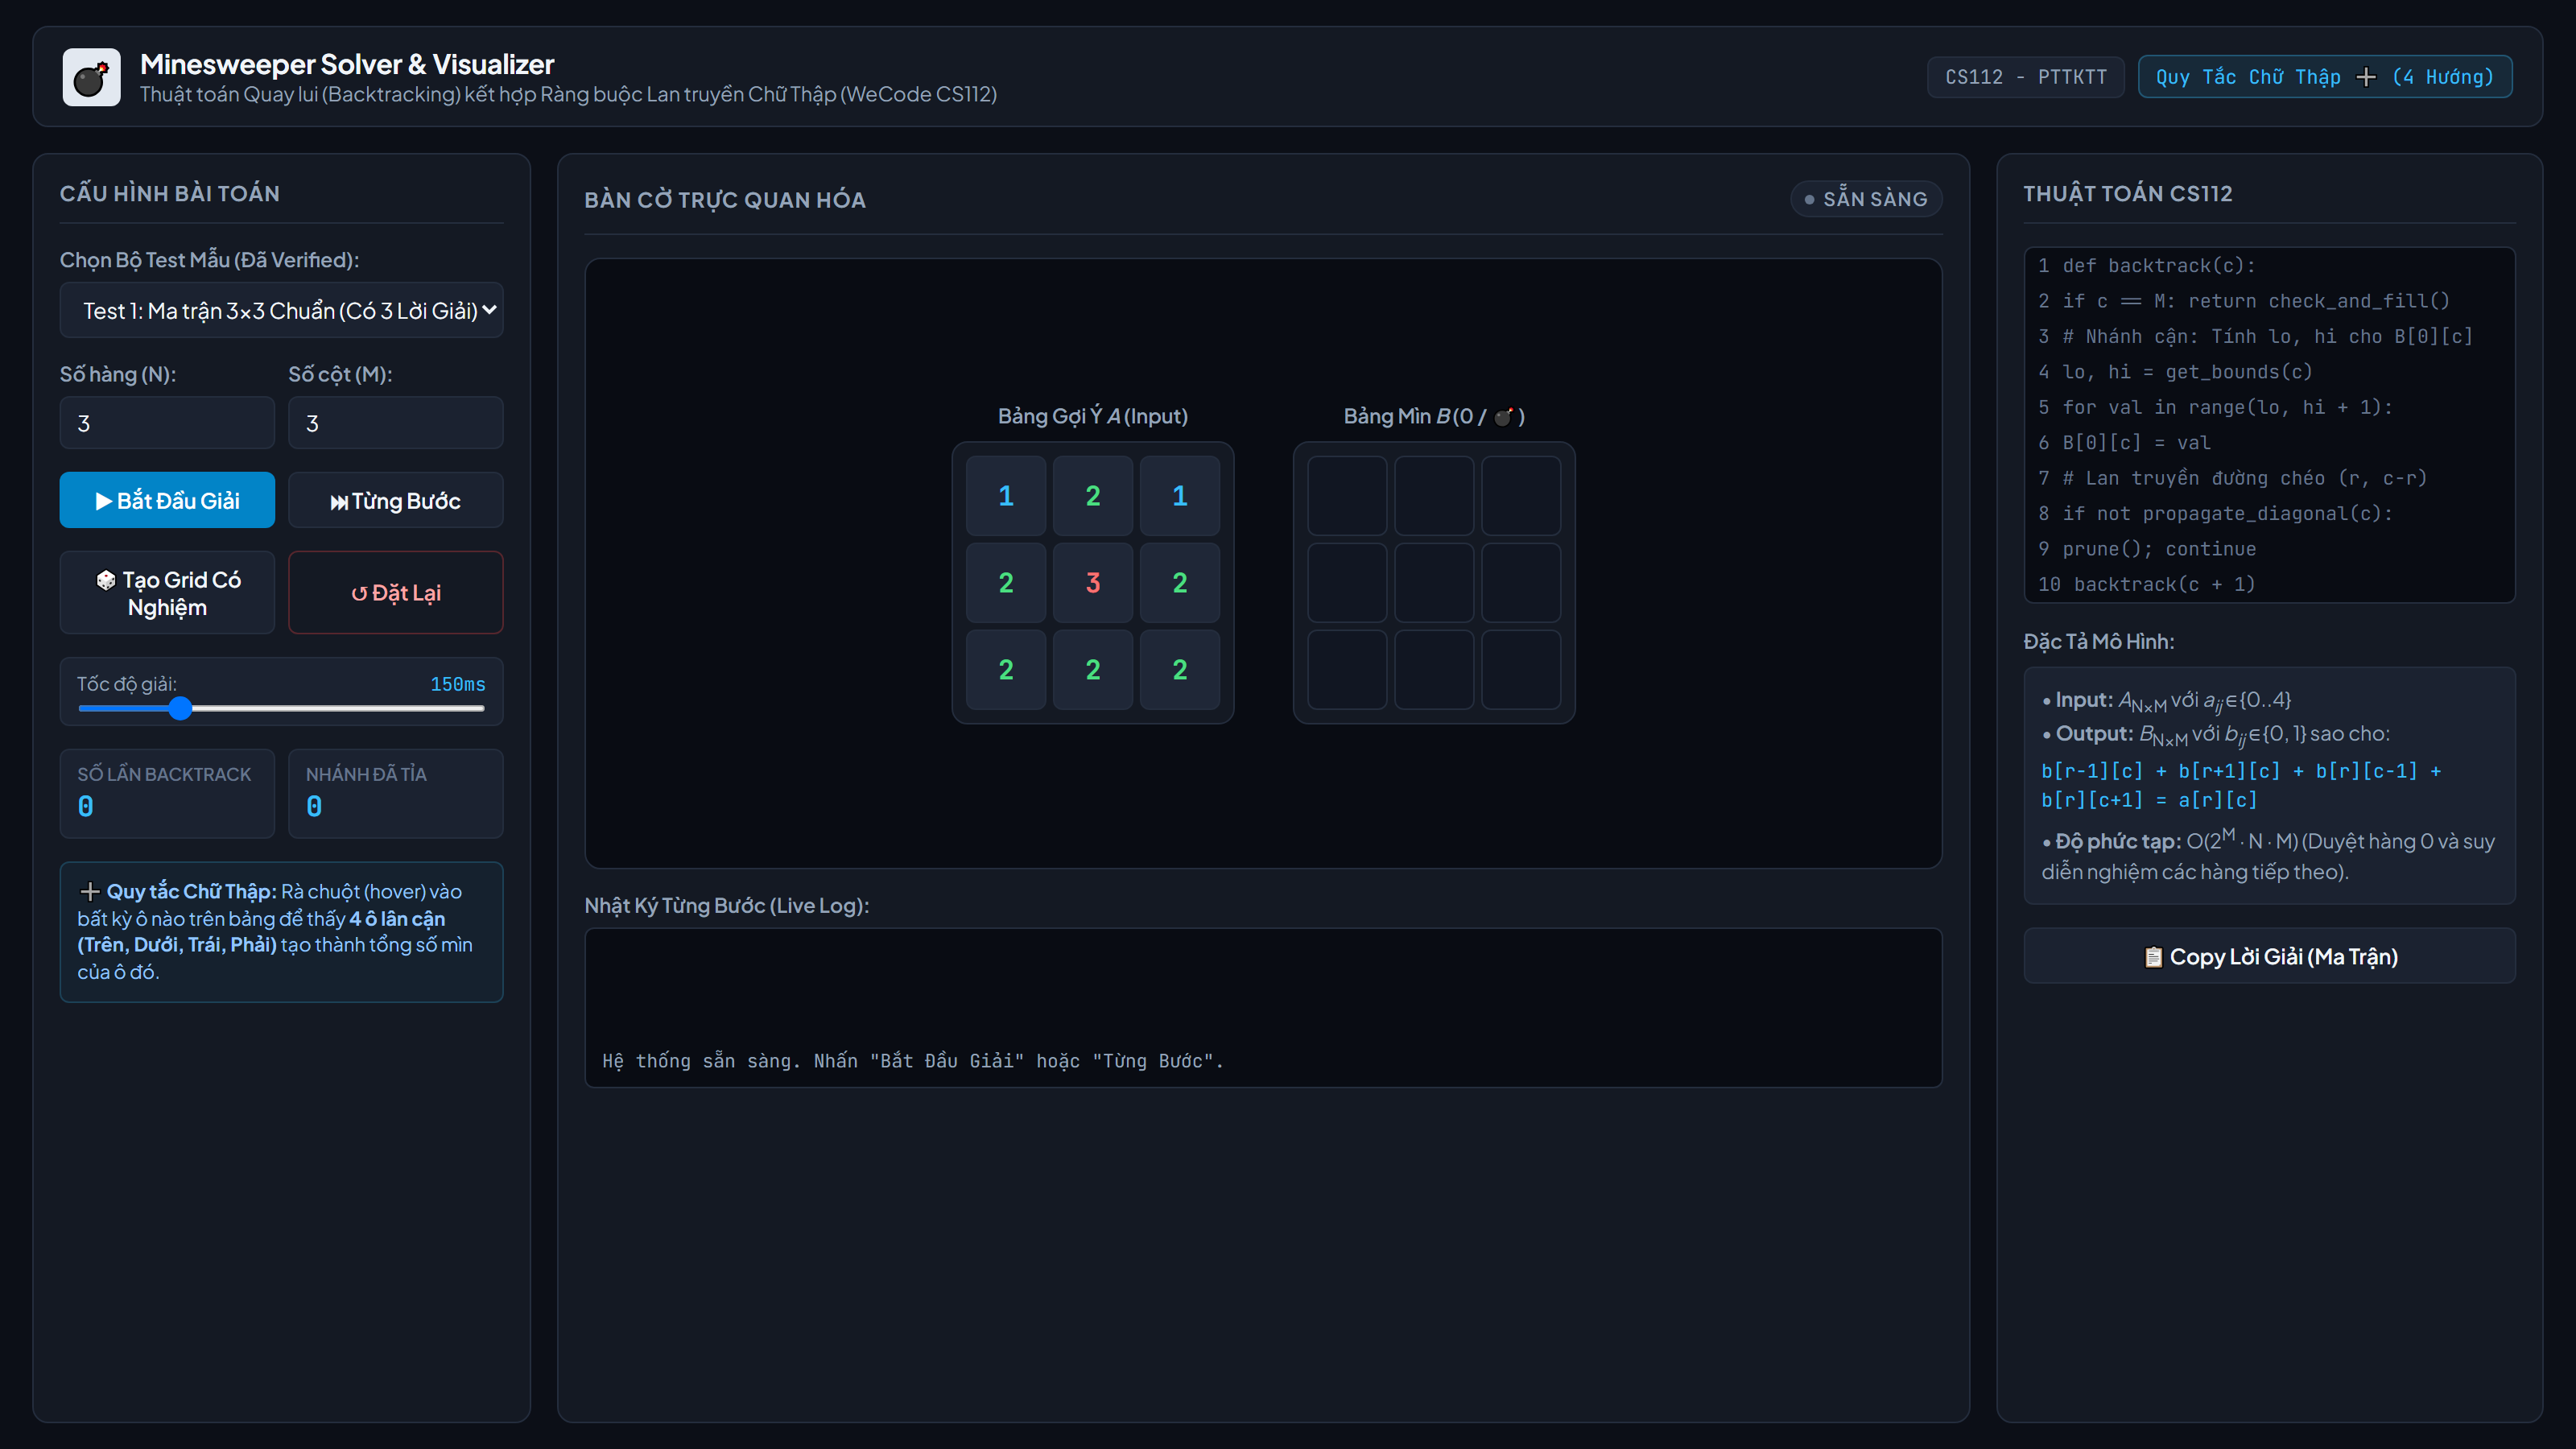
\includegraphics[width=\textwidth]{img/01_overview.png}
    \caption{Giao diện tổng quan: cấu hình (trái), bàn cờ (giữa), mã giả và mô hình (phải).}
\end{figure}

\begin{figure}[H]
    \centering
    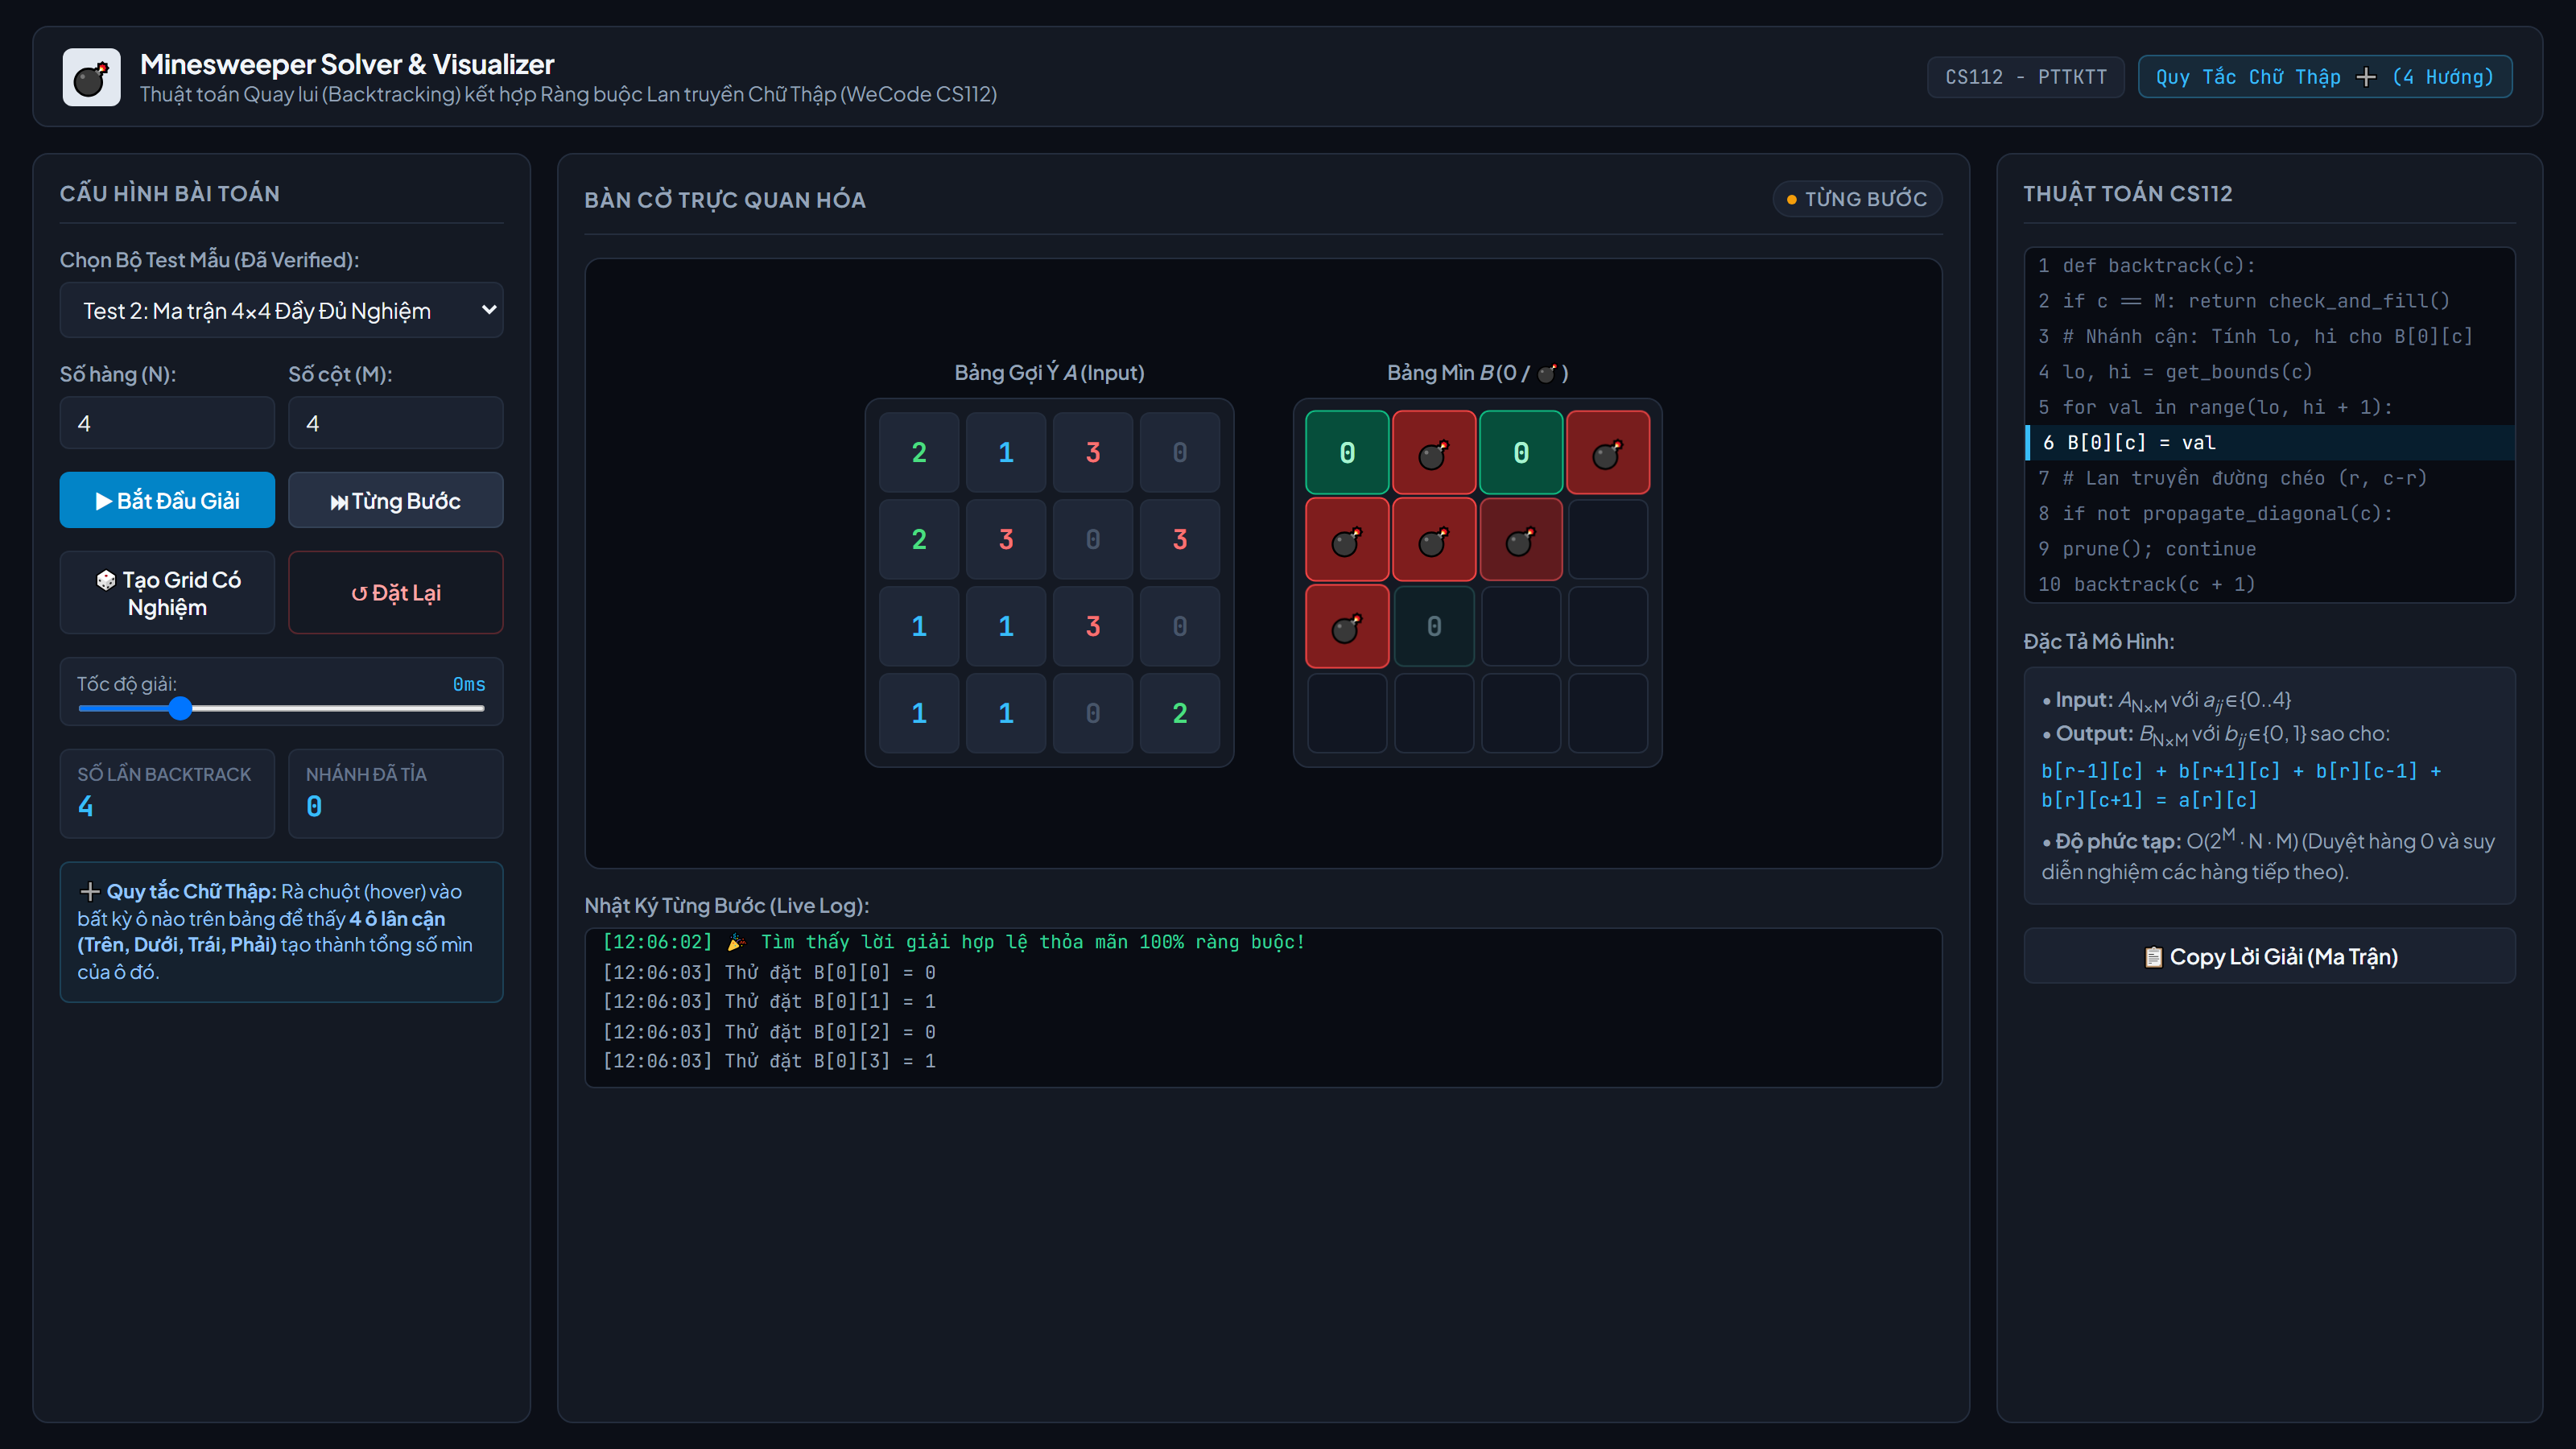
\includegraphics[width=\textwidth]{img/03_step_mode.png}
    \caption{Chế độ từng bước (Test 2): sau khi gán $b_{0,c}$, các ô trên đường chéo $(r, c-r)$ được tính ngay (Cận 2). Dòng mã giả đang chạy được tô sáng.}
\end{figure}

\begin{figure}[H]
    \centering
    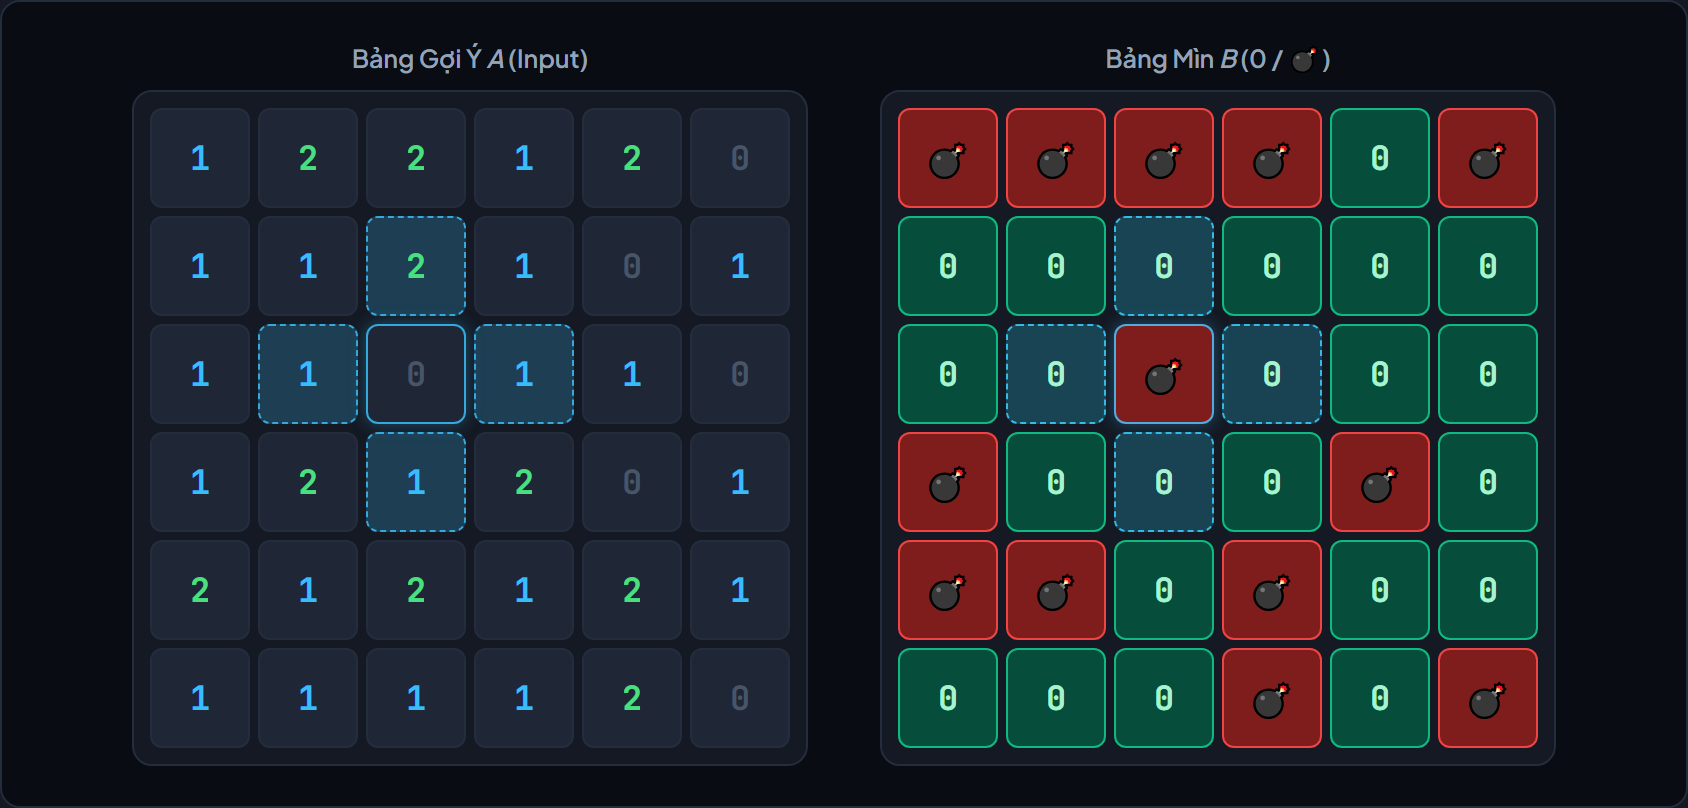
\includegraphics[width=0.85\textwidth]{img/05_cross_verify.png}
    \caption{Lưới ngẫu nhiên $6 \times 6$ đã giải. Rê chuột vào ô $(2,2)$: hình chữ thập được tô sáng trên cả hai bảng.}
\end{figure}

%=====================================================================
\section{Kiểm thử}

\begin{table}[H]
\centering
\begin{tabularx}{\textwidth}{@{}llp{2.8cm}X@{}}
\toprule
\textbf{Test} & \textbf{Kích thước} & \textbf{Kết quả} & \textbf{Ghi chú} \\
\midrule
Test 1 & $3 \times 3$ & Có nghiệm & Có 3 nghiệm, thuật toán dừng ở nghiệm đầu tiên \\
Test 2 & $4 \times 4$ & Có nghiệm & Nghiệm duy nhất \\
Test 3 & $5 \times 5$ & Có nghiệm & Nghiệm duy nhất \\
Test 4 & $3 \times 3$, mọi $a_{ij} = 4$ & Vô nghiệm & Ô góc chỉ có 2 ô kề $\Rightarrow a_{00} \le 2$ \\
Ngẫu nhiên & $1 \times 1$ đến $6 \times 6$ & 200/200 có nghiệm & Không có lần nào báo vô nghiệm sai \\
\bottomrule
\end{tabularx}
\caption{Kết quả kiểm thử. Test 1--3: bản JavaScript cho kết quả trùng khớp với lời giải Python trên WeCode.}
\end{table}

\noindent Cách kiểm thử:
\begin{itemize}
    \item Chạy \texttt{giai\_do\_min\_wecode.py} với các test mẫu, đối chiếu với bản JavaScript.
    \item Chạy mã JavaScript của trang web trong Node.js (không giao diện), gọi đúng hàm điều khiển nút \textit{Bắt Đầu Giải}, mỗi test giải 2 lần liên tiếp để phát hiện lỗi trạng thái.
    \item Sinh 200 lưới ngẫu nhiên có nghiệm, kiểm tra thuật toán luôn tìm được nghiệm.
\end{itemize}

\begin{figure}[H]
    \centering
    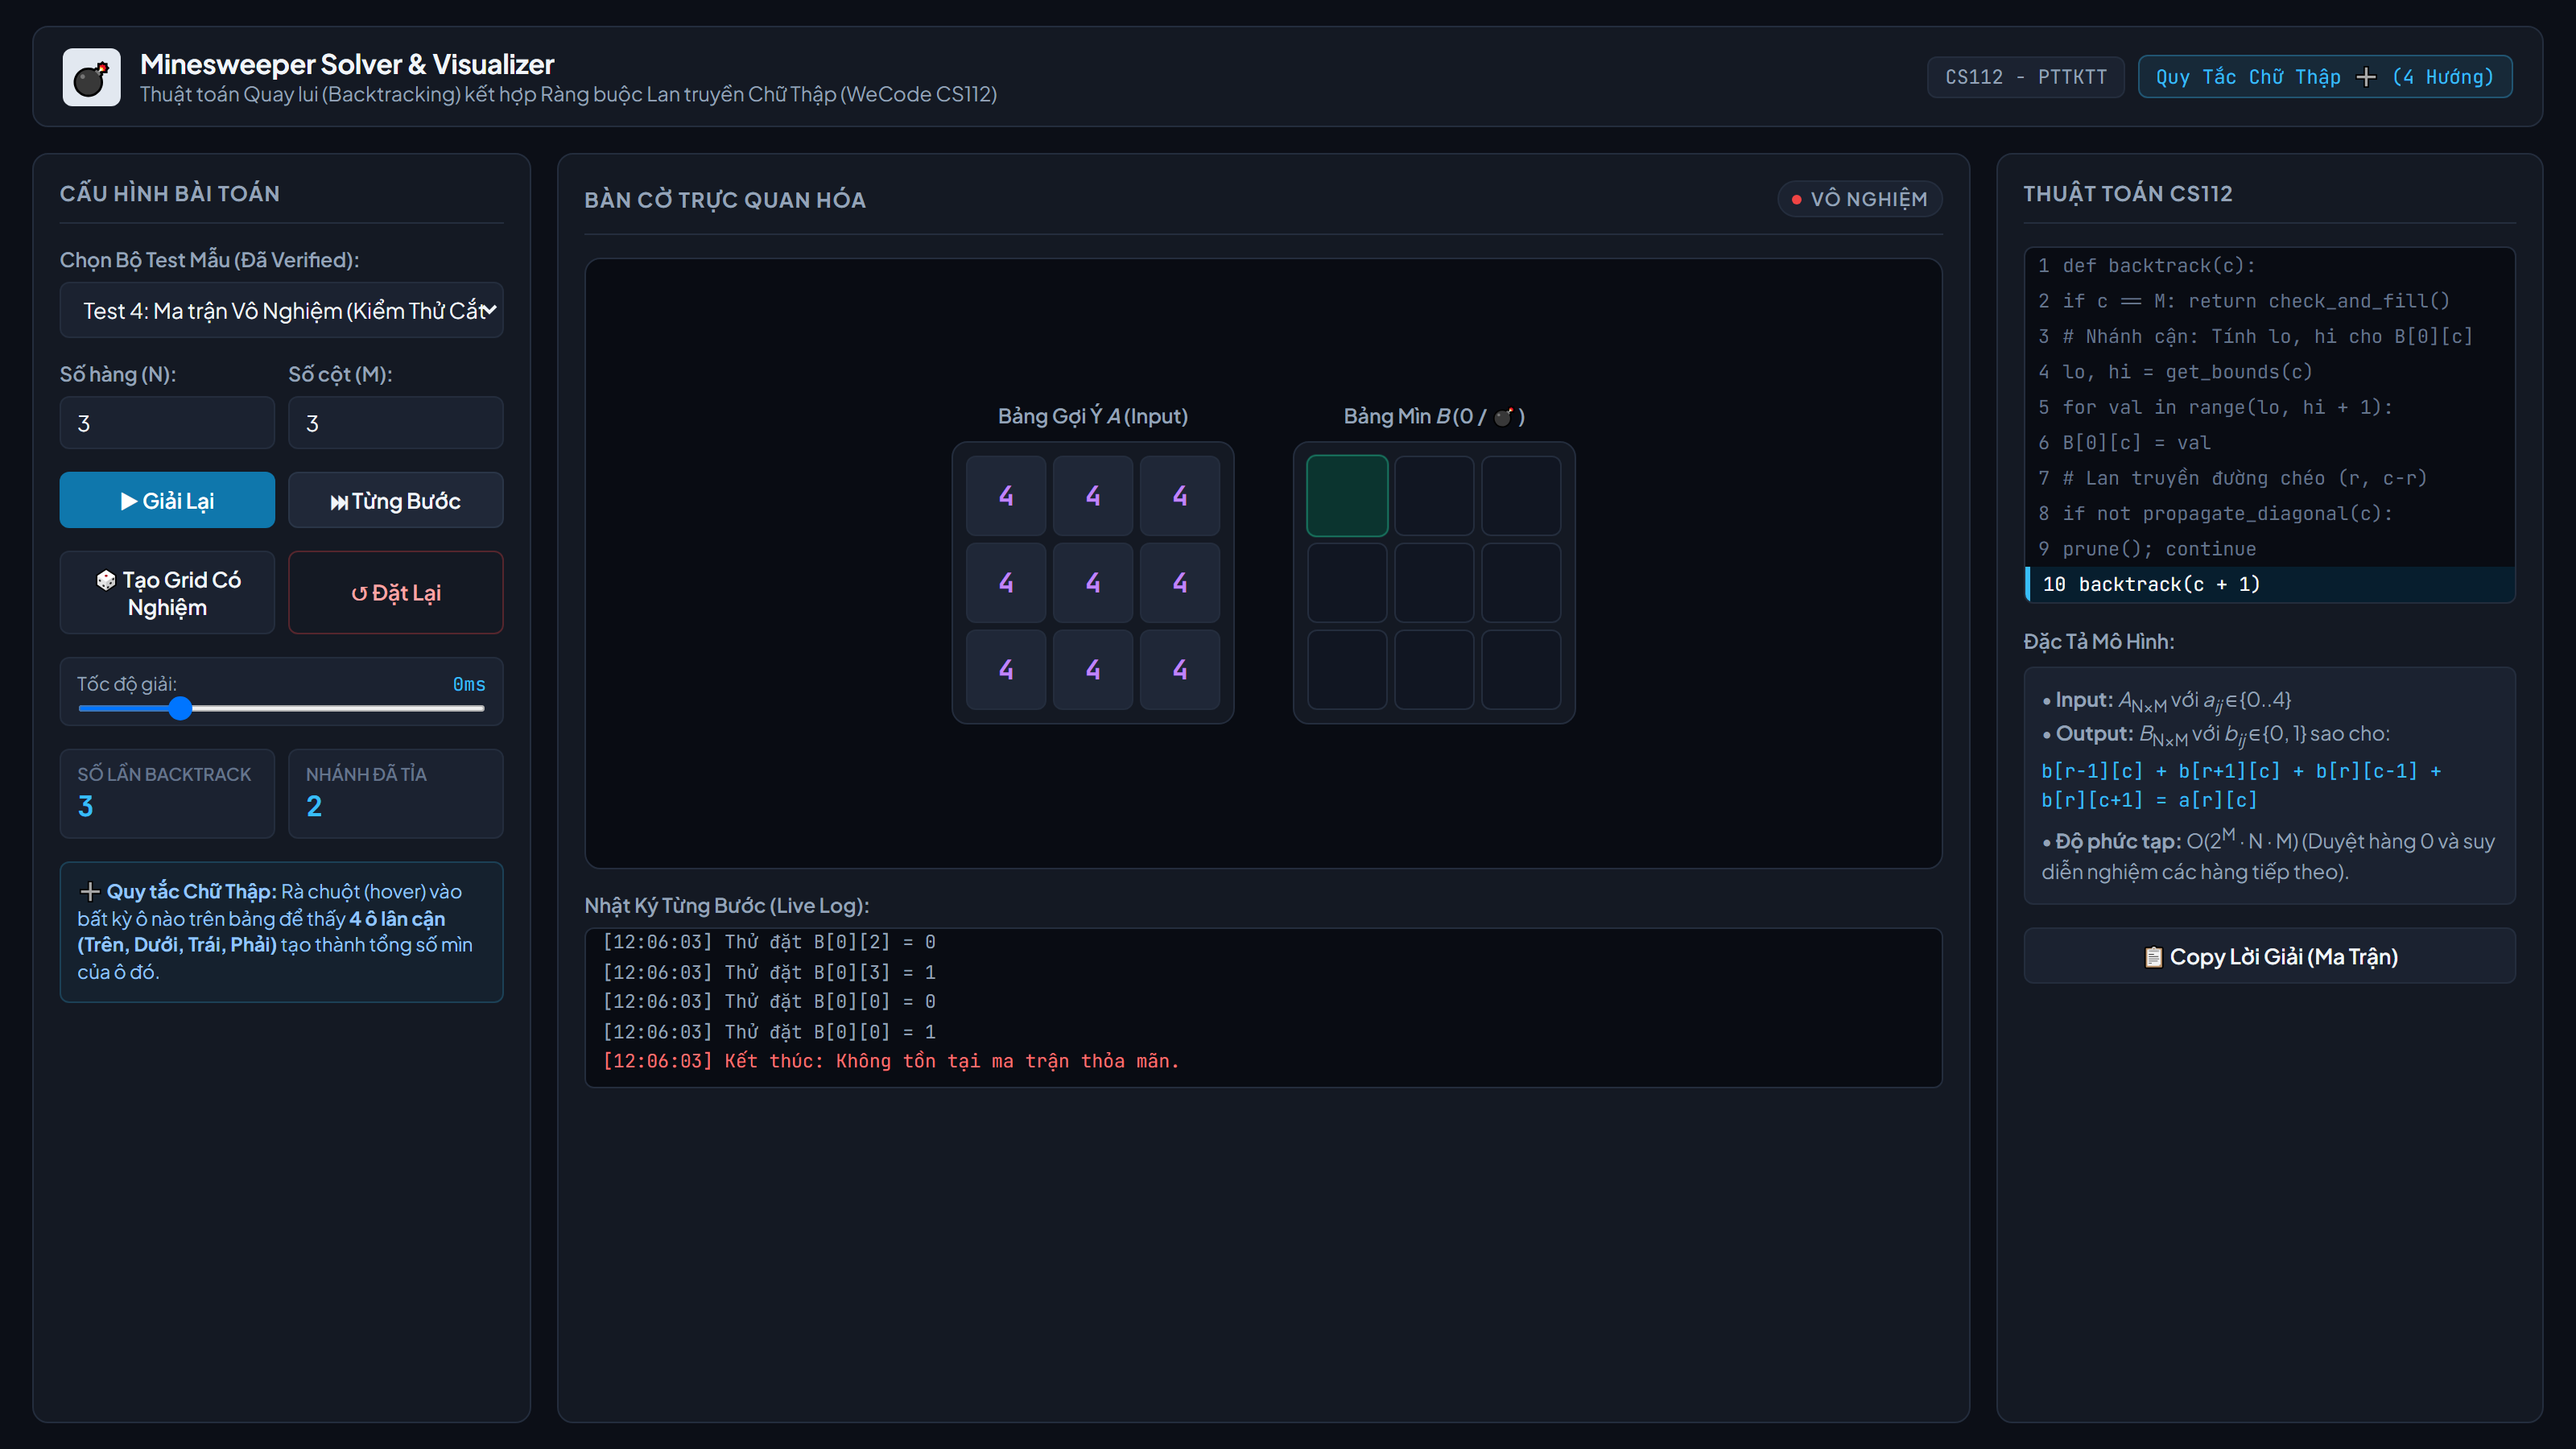
\includegraphics[width=\textwidth]{img/04_no_solution.png}
    \caption{Test 4: thuật toán cắt hết các nhánh và kết luận vô nghiệm.}
\end{figure}

%=====================================================================
\section{Quy trình thực hiện với AI}

\subsection{Công cụ}
\begin{itemize}
    \item \textbf{Antigravity IDE} (trợ lý AI tích hợp trong trình soạn thảo, có quyền đọc/ghi file và chạy lệnh), với các mô hình Gemini 3.1 Pro, Gemini 3.7 Flash và Claude Opus 5.5.
    \item \textbf{Lời giải WeCode} (\texttt{giai\_do\_min\_wecode.py}) có trước khi làm bài tập lớn. \todo{ghi rõ: tự viết / AI hỗ trợ / kết hợp, và đã AC trên WeCode chưa}
\end{itemize}

\subsection{Các bước và yêu cầu (prompt) chính}
\begin{table}[H]
\centering
\small
\begin{tabularx}{\textwidth}{@{}p{0.4cm}p{5.2cm}X@{}}
\toprule
\textbf{\#} & \textbf{Yêu cầu gửi AI} & \textbf{Kết quả} \\
\midrule
1 & ``Trong playlist có buổi cô yêu cầu bài tập lớn là làm gì?'' & AI tìm trong transcript bài giảng: yêu cầu nằm ở Buổi 8 --- ứng dụng có giao diện trực quan hóa, video demo, báo cáo quy trình. \\
2 & ``Nếu chọn bài \texttt{giai\_do\_min\_wecode.py} thì báo cáo thế nào?'' & AI đưa ra 3 phương án (web, Python GUI, dashboard so sánh). Chọn web 1 file. \\
3 & ``ok impl'' & AI dựng bản đầu của \texttt{index.html} và khung báo cáo. \\
4 & ``Giao diện nhìn AI quá và tại sao không có cách giải hợp lệ?'' & Đổi giao diện sang tông tối trung tính, bỏ gradient tím và hiệu ứng kính. Sửa bộ sinh ngẫu nhiên. \\
5 & ``1 số $\to$ chữ thập chứ nhỉ'' & Xác nhận luật 4 ô kề. Thêm hiệu ứng rê chuột hiện hình chữ thập. Thay bộ test mẫu. \\
6 & ``Check lại logic, tại sao lúc vào cũng vô nghiệm'' & AI kiểm thử bằng Node.js, tìm ra lỗi thật (mục 6.3). \\
7 & ``Có cách nào để AI tự quay được không?'' & AI viết script quay video tự động có giọng đọc và phụ đề. \\
\bottomrule
\end{tabularx}
\end{table}

\subsection{Lỗi do AI tạo ra và cách phát hiện, sửa}
\begin{enumerate}
    \item \textbf{Sai luật của đề.} Bản đầu tính số mìn theo \textbf{8 ô xung quanh} (như game Minesweeper gốc), trong khi đề WeCode dùng \textbf{4 ô kề cạnh}. Các bảng sinh ngẫu nhiên vì vậy mâu thuẫn với thuật toán nên luôn ra vô nghiệm. Báo cáo nháp cũng ghi công thức 8 hướng với $a_{ij} \in [0..8]$. \\
    \textit{Phát hiện:} em báo ứng dụng luôn ra vô nghiệm. AI đọc lại mã nguồn WeCode, nhận ra đề chỉ tính 4 ô kề cạnh, sau đó em xác nhận lại luật hình chữ thập. \textit{Sửa:} viết lại bộ sinh ngẫu nhiên và công thức $(\ast)$.

    \item \textbf{Bộ test mẫu vô nghiệm thật.} Test 1 cũ là $\begin{pmatrix}1&1&1\\2&0&2\\1&1&1\end{pmatrix}$. Ô tâm $a_{11} = 0 \Rightarrow b_{01} = b_{10} = 0$, mà $a_{00} = 1$ đòi hỏi $b_{01} + b_{10} = 1$ --- mâu thuẫn. \\
    \textit{Sửa:} sinh các test mẫu từ một $B$ có trước, rồi kiểm chứng bằng lời giải Python.

    \item \textbf{Lỗi trạng thái giao diện.} Giải xong, generator không được hủy. Bấm ``Bắt Đầu Giải'' lần nữa sẽ gọi \texttt{next()} trên generator đã kết thúc, nhận về \texttt{undefined} và báo ``Vô nghiệm'' ngay. Ngoài ra, bấm ``Từng Bước'' khi đang chạy tự động làm hai luồng chạy chồng lên nhau. \\
    \textit{Phát hiện:} chạy thuật toán JavaScript độc lập trong Node.js thì ra đúng, chứng tỏ lỗi nằm ở phần điều khiển chứ không ở thuật toán. \textit{Sửa:} hủy generator khi kết thúc, khóa nút từng bước khi đang chạy, đặt lại khi người dùng sửa ô gợi ý.

    \item \textbf{Ký hiệu LaTeX hiện thô trên giao diện.} Chuỗi như \verb|$A_{N \times M}$| được ghi thẳng vào HTML. Trình duyệt không hiểu LaTeX nên hiện nguyên ký tự. \\
    \textit{Phát hiện:} xem lại từng khung hình của video demo. \textit{Sửa:} dùng ký hiệu HTML (\texttt{<sub>}, \texttt{<sup>}, $\times$, $\in$).
\end{enumerate}

\subsection{Nhận xét}
AI làm nhanh phần giao diện, hiệu ứng và kịch bản quay video. Tuy nhiên AI đã \textbf{tự tin đưa ra kết quả sai} ở những chỗ cần hiểu đúng đề (8 hướng thay vì 4 hướng) và ở bộ dữ liệu test. Những lỗi này chỉ lộ ra khi đối chiếu với đề và \textbf{chạy kiểm thử thực tế}, không thể phát hiện chỉ bằng cách đọc code. \\
\todo{Thêm nhận xét cá nhân: phần nào em tự hiểu/tự kiểm tra, điều em học được}

%=====================================================================
\section{Kết luận}
\begin{itemize}
    \item Đưa bài toán từ $2^{NM}$ phương án về $2^M$ nhờ nhận xét hàng $0$ quyết định toàn bộ bảng, kết hợp 2 cận cắt nhánh sớm. Độ phức tạp $O(2^M \cdot NM)$.
    \item Ứng dụng web cho phép quan sát từng bước gán, cắt nhánh, quay lui, và kiểm tra trực quan ràng buộc hình chữ thập.
    \item Hướng phát triển: chuyển vị bảng để quay lui trên cạnh ngắn hơn; liệt kê \textbf{tất cả} nghiệm thay vì dừng ở nghiệm đầu tiên.
\end{itemize}

\end{document}
